%
% A simple LaTeX template for Books
%  (c) Aleksander Morgado <aleksander@es.gnu.org>
%  Released into public domain
%
\RequirePackage{lineno} 
\documentclass{article}
\usepackage[a4paper, top=3cm, bottom=3cm]{geometry}
%\usepackage[latin1]{inputenc}
%\usepackage{setspace}
\usepackage{fancyhdr}
%\usepackage{tocloft}
\usepackage{verbatim}
\usepackage{graphicx,amsmath,epsfig,color,amsfonts,relsize,subfigure}
\usepackage{authblk}
%\usepackage[running]{lineno}
\newcommand{\fbinv} {\mbox{\ensuremath{\,\text{fb}^\text{$-$1}}}}
\begin{document}

 
\pagestyle{empty}
\pagenumbering{}
% Set book title
\title{\textbf{W$\gamma$ at $\sqrt{s}=$8~TeV.}}

\author[1]{Lovedeep}
\author[1]{Yurii}
\author[1]{Sachiko}
\author[2]{Katya}
\author[2]{Ilya}
\author[3]{Yutaro}

\affil[1]{Kansas State University, Manhattan}
\affil[2]{University of Nebraska-Lincoln, USA}
\affil[3]{Carnegie Melon University, USA}
\maketitle

\begin{abstract}
We present a study of W$\gamma$ production in proton-proton
collisions at $\sqrt{s} = 8$~TeV. 
\end{abstract}

% 2nd page, thanks message
%-------------------------------------------------------------------------------
\thispagestyle{empty}
\newpage


% General definitions for all Chapters
%-------------------------------------------------------------------------------

% Define Page style for all chapters
\pagestyle{fancy}
% Delete the current section for header and footer
\fancyhf{}
% Set custom header
\lhead[]{\thepage}
\rhead[\thepage]{}

% Set arabic (1,2,3...) page numbering
\pagenumbering{arabic}
\tableofcontents

%
% Not enumerated chapter
%-------------------------------------------------------------------------------
\linenumbers
\clearpage
\section{Introduction}
\label{sec:intro}
The Standard Model (SM) has been proved to be an accurate description 
of production of elementary particles observed so far. The interaction of W bosons
with photons is particularly important as a important test of self coupling 
of these bosons as predicted by non-Abelian gauge group of electroweak sector. Precise measurements of diboson properties and cross 
sections are a crucial step towards understanding the production of major 
backgrounds of Higgs boson searches at LHC. 

In this analysis note we report the analysis of inclusive $W\gamma + X$  processes  
using  leptonic decays of $W\to \ell\nu$ where $\ell = e, \mu$. 
The $W\gamma$ productions at tree level can be represented by Feynman diagrams in 
Figs.~\ref{fig:feynman_wg}~and~\ref{fig:feynman_zg} 
as three processes: initial state radiation (ISR) where a photon is produced from one of 
the incoming partons, final state radiation (FSR) where a photon is radiated off one of 
the charged leptons from the $W$ boson decay, and finally when a photon is produced in 
$s-$channel via TGC $WW\gamma$ for $W\gamma$ production.  The last process is allowed only for $W\gamma$g production in the SM, as there are no neutral TGC in the SM.
\begin{figure}[htb]
\begin{center}
{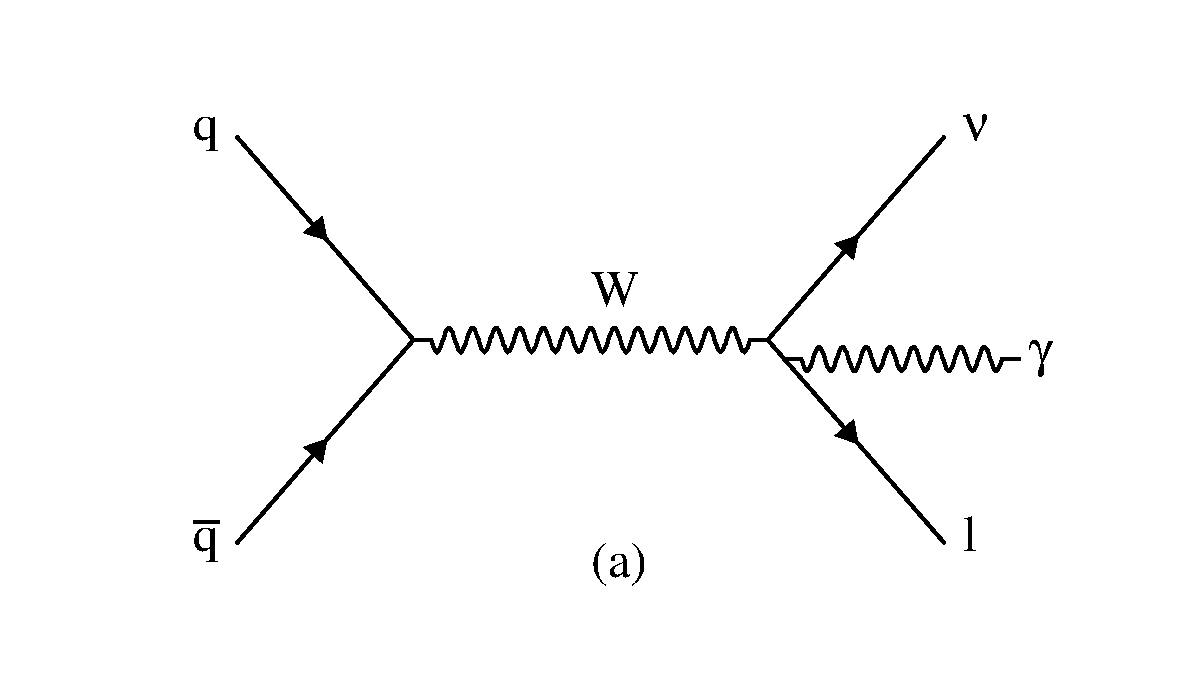
\includegraphics[width=0.49\textwidth]{figs/wg_fsr}}
{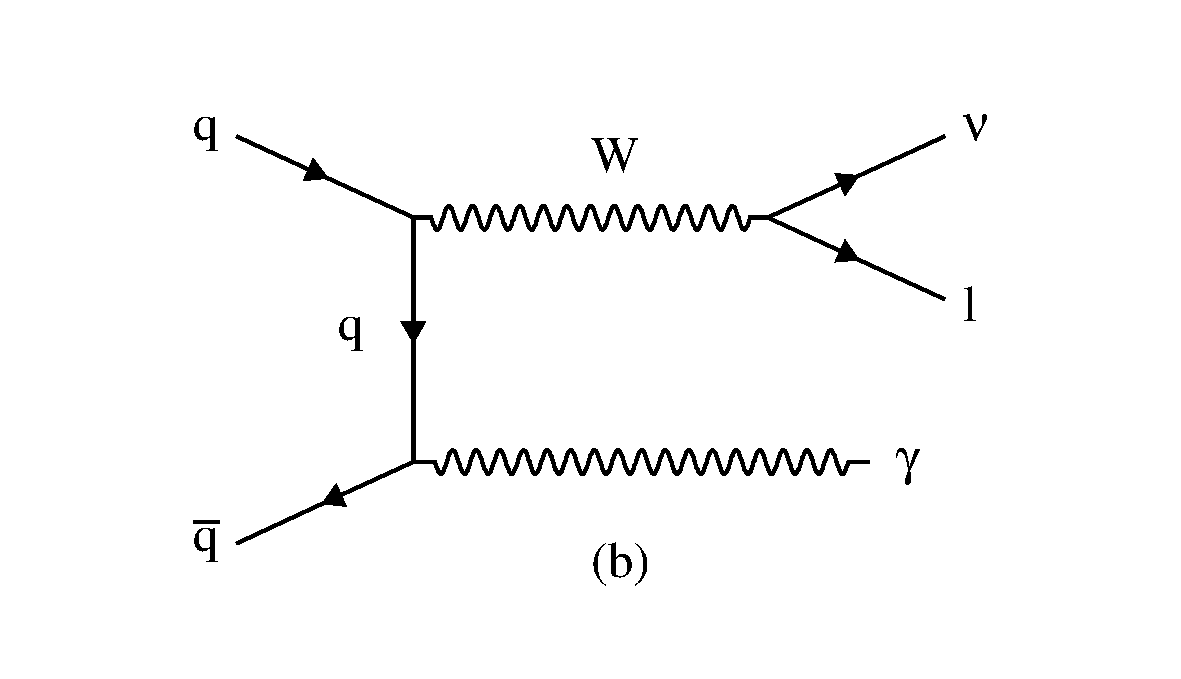
\includegraphics[width=0.49\textwidth]{figs/wg_isr}}
{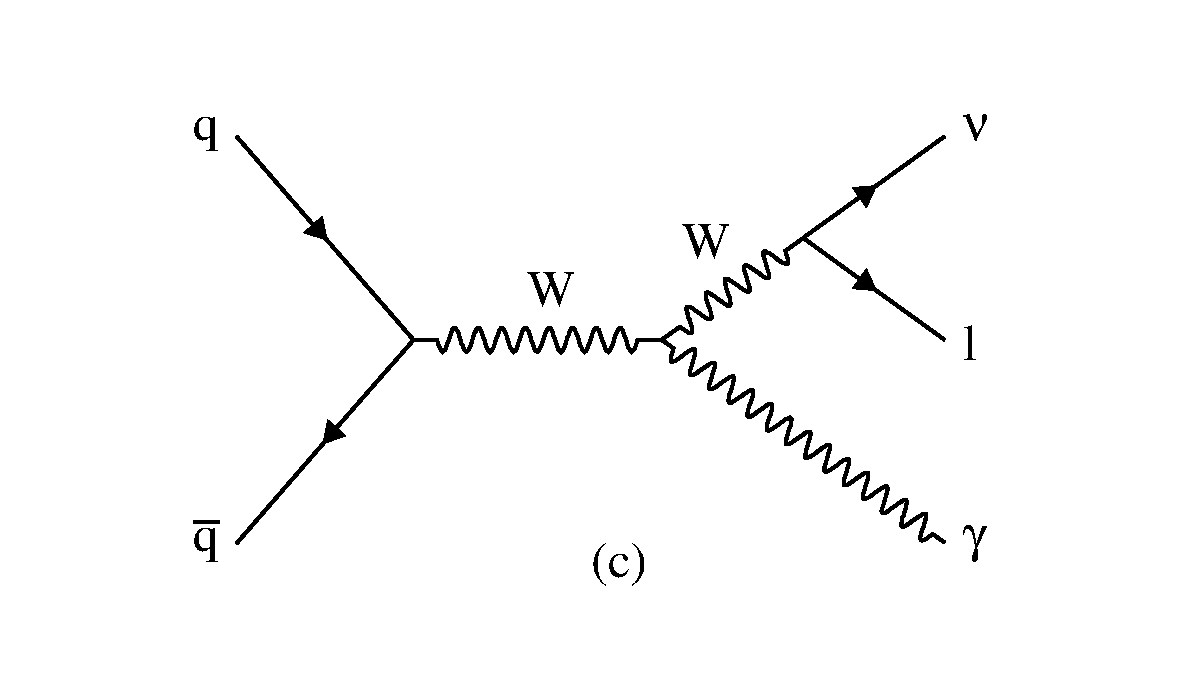
\includegraphics[width=0.49\textwidth]{figs/wg_wwg}}
\caption{Feynman diagrams of the W$\gamma$ production via 
final (a) and initial (b) state radiation and via WW$\gamma$ 
trilinear gauge coupling (c).}
\label{fig:feynman_wg}
\end{center}
\end{figure}


\section{Data and Monte Carlo samples}
\label{sec:DataAndMC}

\subsection{Data sample}
The data sample we use in this analysis was recorded by the CMS experiment 
in 2012. The data is collected by single electron ($p_T>27$GeV) triggers~\ref{tab:triggers}. 
Only certified runs and luminosity sections are considered, which 
means that good functioning of all CMS sub-detectors is required.
The selection of the validated run and luminosity sections are obtained from the following official JSON file:
\begin{itemize}
\item{\small{Cert$\_$190456$-$208686$\_$8TeV$\_$22Jan2013ReReco$\_$Collisions12$\_$JSON.txt}}
\end{itemize}
 The total 
statistics analyzed correspond to an integrated luminosity of 19.6~\fbinv.

\begin{table}[htbp]
  \begin{center}
 {\small
  \begin{tabular} {l|l|c}
\hline
  Dataset & Trigger name & Description\\
  \hline \hline
  SingleElectron & HLT\_Ele27\_WP80*        & $p_T>27~GeV$ \\
  \hline
  \end{tabular}
}
  \caption{Analysis triggers for data sample.\label{tab:triggers}}
  \end{center}
\end{table}

The dataset used for the analysis and the corresponding run ranges are 
listed in Table~\ref{tab:datasets}. All samples have been processed using a 
\texttt{CMSSW\_5\_3\_2} release version.

\begin{table}[]
  \begin{center}
  \begin{tabular}{r|r}
  \hline
  Dataset name & Run range \\
  \hline
  /SingleElectron/Run2012A-22Jan2013-v1/AOD   &  190456-193621           \\
  \hline
  /SingleElectron/Run2012B-22Jan2013-v1/AOD   &   193833-196531       \\
  \hline
  /SingleElectron/Run2012C-22Jan2013-v1/AOD & 198022-203746\\
  \hline
  /SingleElectron/Run2012D-22Jan2013-v1/AOD  & 203777-208686 \\
  
  \hline
  \hline
  \end{tabular}
  \end{center}
  \caption{Summary of data samples used and run ranges of applicability.}
  \label{tab:datasets}
\end{table}%
\subsection{Monte Carlo samples}

All MC samples considered in this analysis come from the official
``Summer12\_53X''.  Events from all samples were
reconstructed making use of a \texttt{CMSSW\_5\_3\_X} release version.
The simulated samples are reweighted to represent the distribution of the
number of pp interactions per bunch crossing (pile-up), as measured in
the data.



Information on Monte Carlo samples used for the analyses is given in 
Table~\ref{tab:mc_bkg_samples} 
for signals and backgrounds. 
The corresponding leading order (LO) and next-to-leading order (NLO) 
cross sections are also listed in this Table.



\begin{table}[h]
  \scriptsize
  \begin{center}
    \caption{Summary of Monte Carlo background samples used.}
    \begin{tabular}{|l|l|l|}
      \hline
      Process (Fall11)                     & $\sigma$, pb        & Dataset Name (AODSIM data tier) \\ \hline
      $W\gamma \rightarrow l\nu\gamma$     & 553.92 (NLO)         & \verb /WGToLNuG_TuneZ2star_8TeV-madgraph-tauola \\
      $W \rightarrow l\nu + jets$          & 36257.2 (NNLO)        & \verb /WJetsToLNu_TuneZ2Star_8TeV-madgraph-tarball \\ 
      $Z \rightarrow ll + jets$            & 3503.71         & \verb /DYJetsToLL_M-50_TuneZ2Star_8TeV-madgraph-tarball \\
      $t\bar{t} + jets+1l$                    & 99.44 (NNLO)          & \verb /TTJets_SemiLeptMGDecays_8TeV-madgraph  \\
      $t\bar{t} + jets+2l$                    & 23.83           & \verb /TTJets_FullLeptMGDecays_8TeV-madgraph \\
      $t\bar{t} + \gamma$                    & 1.444           & \verb /TTGJets_8TeV-madgraph \\
      $Z\gamma \rightarrow ee\gamma$       & 159.120          & \verb /ZGToLLG_8TeV-madgraph \\
      \hline
    \end{tabular}
    \label{tab:mc_bkg_samples}
  \end{center}
\end{table} 



\section{Object selection}
\label{sec:ObjectSelection}
In this Section we document the electron, 
and photon identification and isolation criteria, MET criteria, and provide the
results of comparing Monte Carlo simulation with data.


\subsection{Electron selection}
\label{sec:eid}
In $W\gamma$ analysis we consider electrons with $p_T > 30$~GeV and passing
the Medium-identification and isolation optimized by EGamma-POG for 2012 analyses.
We summarize electron identification and isolation requirements in Table~\ref{}.

The ECAL fiducial region is defined in terms of barrel and endcap
sections with pseudorapidity ranges of $|\eta| < 1.4442$ and  
$1.566 < |\eta| < 2.5$, respectively. An electron is considered
to be within this ECAL acceptance if its associated SuperCluster (SC) is
within the ECAL acceptance.
Data/MC scale factors are applied.


\subsection{Photon selection}
Photon candidates are reconstructed as SuperClusters with 
$E_{T} > 15$~GeV in the fiducial volume of the ECAL detector:
barrel (EB) with $|\eta|<1.4442$ and endcap (EE) with 
$1.566 < |\eta| < 2.5$. To reduce copious background objects from jets misidentified as photons 
we apply the Medium identification and isolation selections as recommended by EGamma-POG.
Data/MC scale factors are applied.

\subsection{MET}
no selection yet


\clearpage



\end{document}
